% -*- TeX -*- -*- UK -*- -*- BMR -*-
% ----------------------------------------------------------------
% Beamer presentation ************************************************
% **** -----------------------------------------------------------
\documentclass{beamer}%[hyperref={backref=slide}]

\input{sl_slide_preamble.tex}
%\input{sl_slide_preamble_nonotes.tex}
\input{sl_slide_graphics_preamble.tex}
\input{sl_definitions.tex}
\input{sl_slide_symbols.tex}
%
\graphicspath{{"Figs/"}}
\DeclareMathOperator{\SNR}{SNR}
\DeclareMathOperator{\snr}{SNR}
%matrices
\newcommand{\inv}{^{-1}}
\newcommand{\I}{\mathbf{I}}
%prob vector
\newcommand{\pr}{\mathbf{p}}
%equilibrium distribution
\newcommand{\eq}{\pr^\infty}
%first passage times
\newcommand{\fpt}{\mathbf{T}}
%off-diag first passage times
\newcommand{\fptb}{\overline{\fpt}}
%other symbols
\newcommand{\w}{\mathbf{w}}
\newcommand{\W}{\mathbf{W}}
\newcommand{\frg}{\W^\mathrm{F}}
\newcommand{\M}{\mathbf{M}}
\newcommand{\F}{\boldsymbol{\Phi}}
\newcommand{\wv}{\vec{w}}
%super/subscripts
\newcommand{\pot}{^{\text{pot}}}
\newcommand{\dep}{^{\text{dep}}}
\newcommand{\potdep}{^{\text{pot/dep}}}
\newcommand{\lmax}{_{\text{max}}}
\newcommand{\lmin}{_{\text{min}}}
%quantities
\newcommand{\initial}{\mathcal{I}}
\newcommand{\area}{\mathcal{A}}
\newcommand{\CS}{\mathcal{S}}
\newcommand{\comp}{^\mathrm{c}}
\renewcommand{\e}{\mathsf{e}}
%---------Title-----------------------------------------------------------

\title[Impaired learning with enhanced plasticity]{A saturation model for impaired learning with enhanced plasticity}
%
\subtitle{\small{based on work in preparation by: T.D. Barbara Nguyen-Vu, Grace Q. Zhao, Han-Mi Lee, SL, Surya Ganguli, Carla J. Shatz, Jennifer L. Raymond
}}
%
\author{Subhaneil Lahiri%\inst{1}
}
%
\institute[Stanford]{%
%\inst{1}
Stanford University, Applied Physics
}
%
%\slideCaption{}

%---------Beginning--------------------------------------------------------

\begin{document}

%-------------Slide--------------------------------------------------------

\begin{frame}
%
 \titlepage
%
\end{frame}

%-------------Slide--------------------------------------------------------

\begin{frame}{Outline}
%
 \tableofcontents[hideallsubsections]
 %
%
\end{frame}


%-------------Section--------------------------------------------------------

\section{VOR learning and the cerebellum}

%-------------Section--------------------------------------------------------

\section{The effects of enhanced plasticity and saturation}


%-------------Slide--------------------------------------------------------

\begin{frame}{Questions}
%
 \begin{itemize}
   \item Can we find a purely synaptic explanation of these results?
   \item Can the saturation effect overcome the enhanced plasticity?
   \item How can a little reverse bias help, but too much hurt?
 \end{itemize}
%
\end{frame}

%-------------Section--------------------------------------------------------

\section{Modelling approach}

%-------------Section--------------------------------------------------------

\section{Modelling results}


%-------------Slide--------------------------------------------------------

\begin{frame}{Binary synapse}
%
 %
 \begin{center}
   \includegraphics[width=0.15\linewidth]{binary.svg} \\[1cm]
   \aligntop{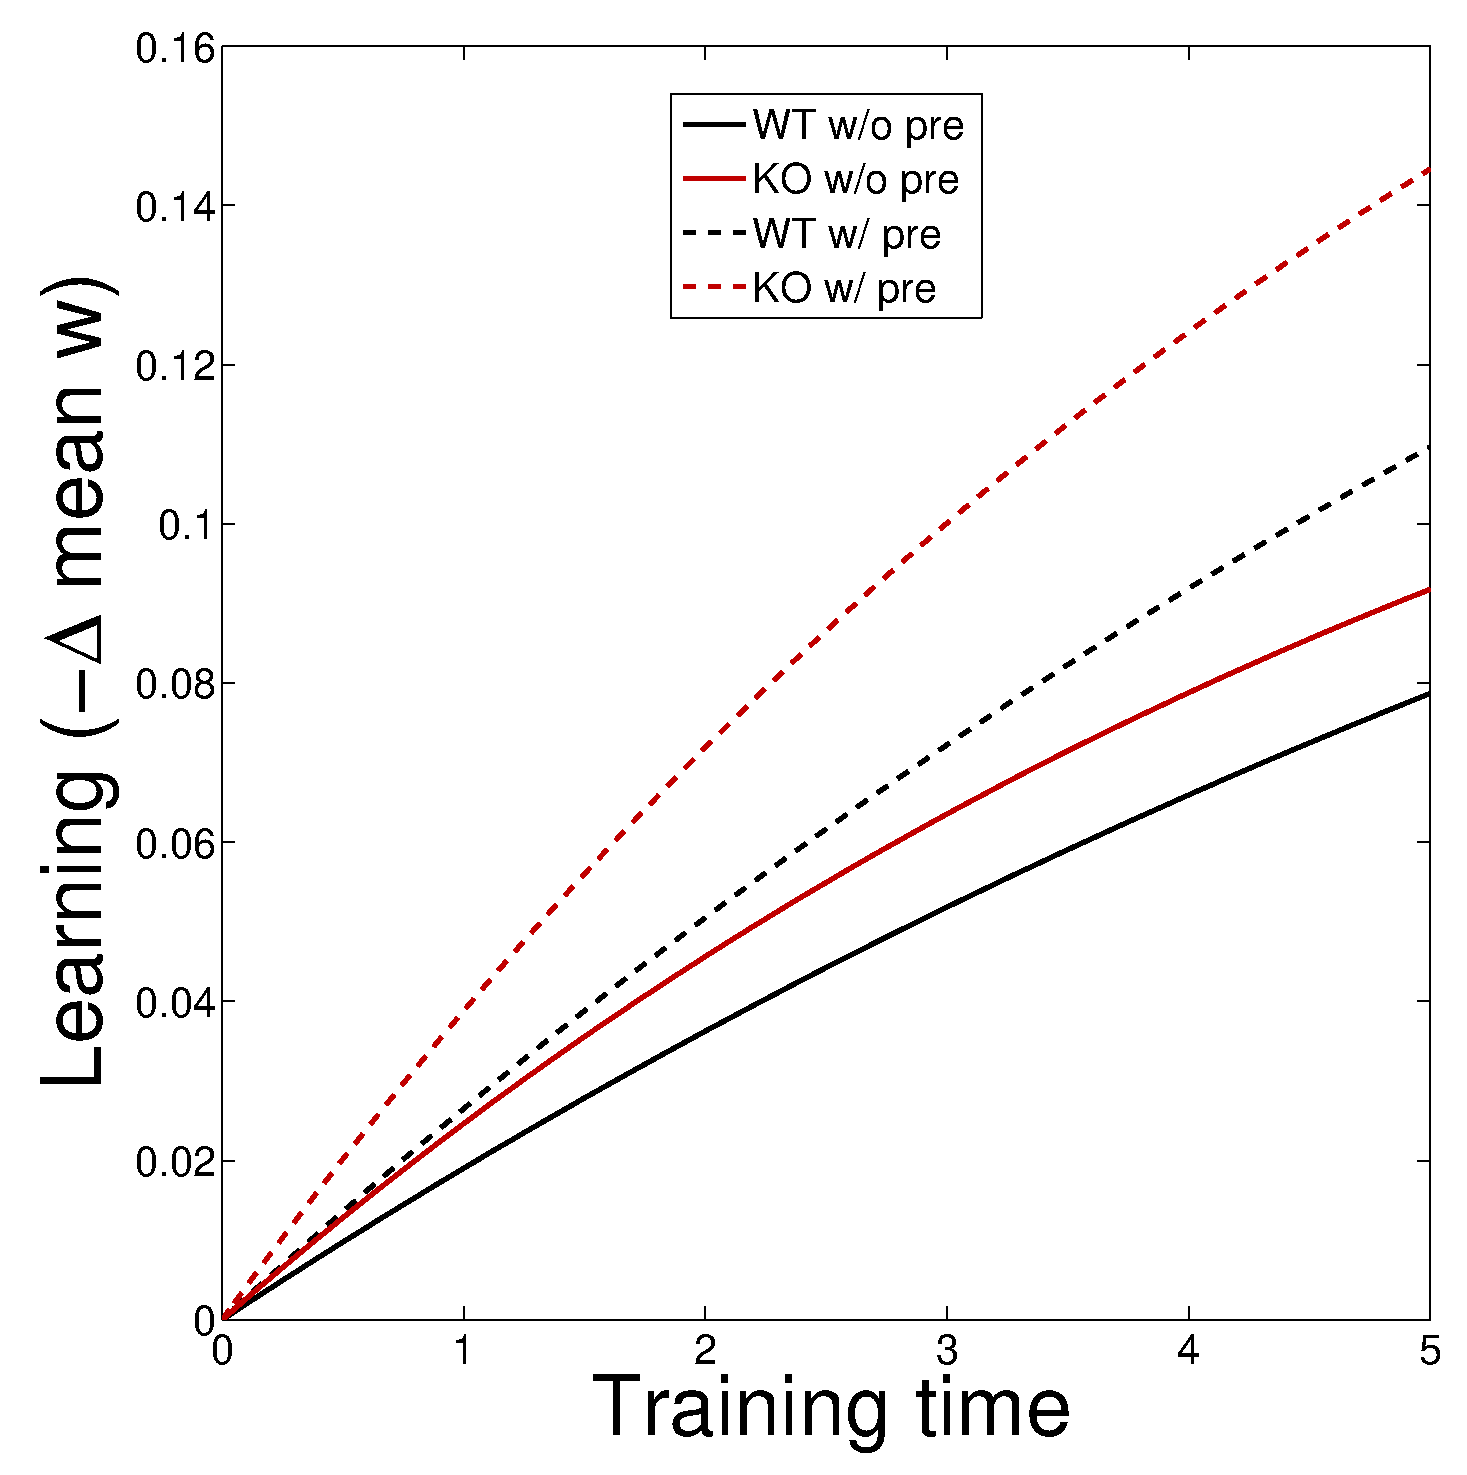
\includegraphics[width=0.35\linewidth]{binary_learnS.eps}}
   \hspace{2cm}
   \aligntop{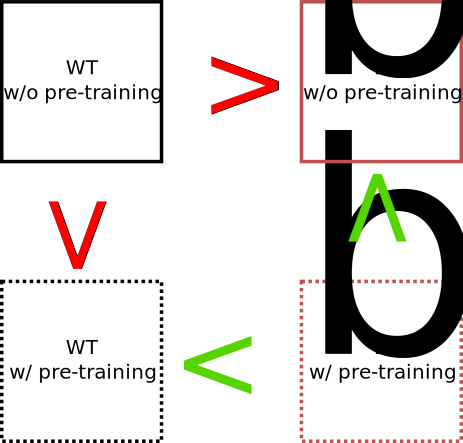
\includegraphics[width=0.35\linewidth]{comparisons_binary.svg}}
 \end{center}
 %
 \note[item]{understand why next slide}
%
\end{frame}

%-------------Slide--------------------------------------------------------

\begin{frame}{Binary synapse: initial distributions}
%
 %
 \begin{center}
 \begin{tabular}{ll}
   \aligntop{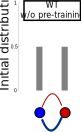
\includegraphics[height=0.25\linewidth]{binary_bar_wt_wo.svg}}
   \hspace{2cm} &
   \aligntop{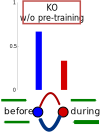
\includegraphics[height=0.25\linewidth]{binary_bar_ko_wo.svg}}
   \\[3cm]
   \aligntop{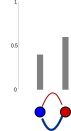
\includegraphics[height=0.25\linewidth]{binary_bar_wt_w.svg}}
   &
   \aligntop{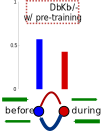
\includegraphics[height=0.25\linewidth]{binary_bar_ko_w.svg}}
 \end{tabular}
 \end{center}
 %
 \note[item]{understand why next slide}
%
\end{frame}

%-------------Slide--------------------------------------------------------

\begin{frame}{Serial synapse}
%
 %
 \begin{center}
   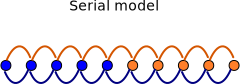
\includegraphics[width=0.5\linewidth]{serial.svg} \\[1cm]
   \aligntop{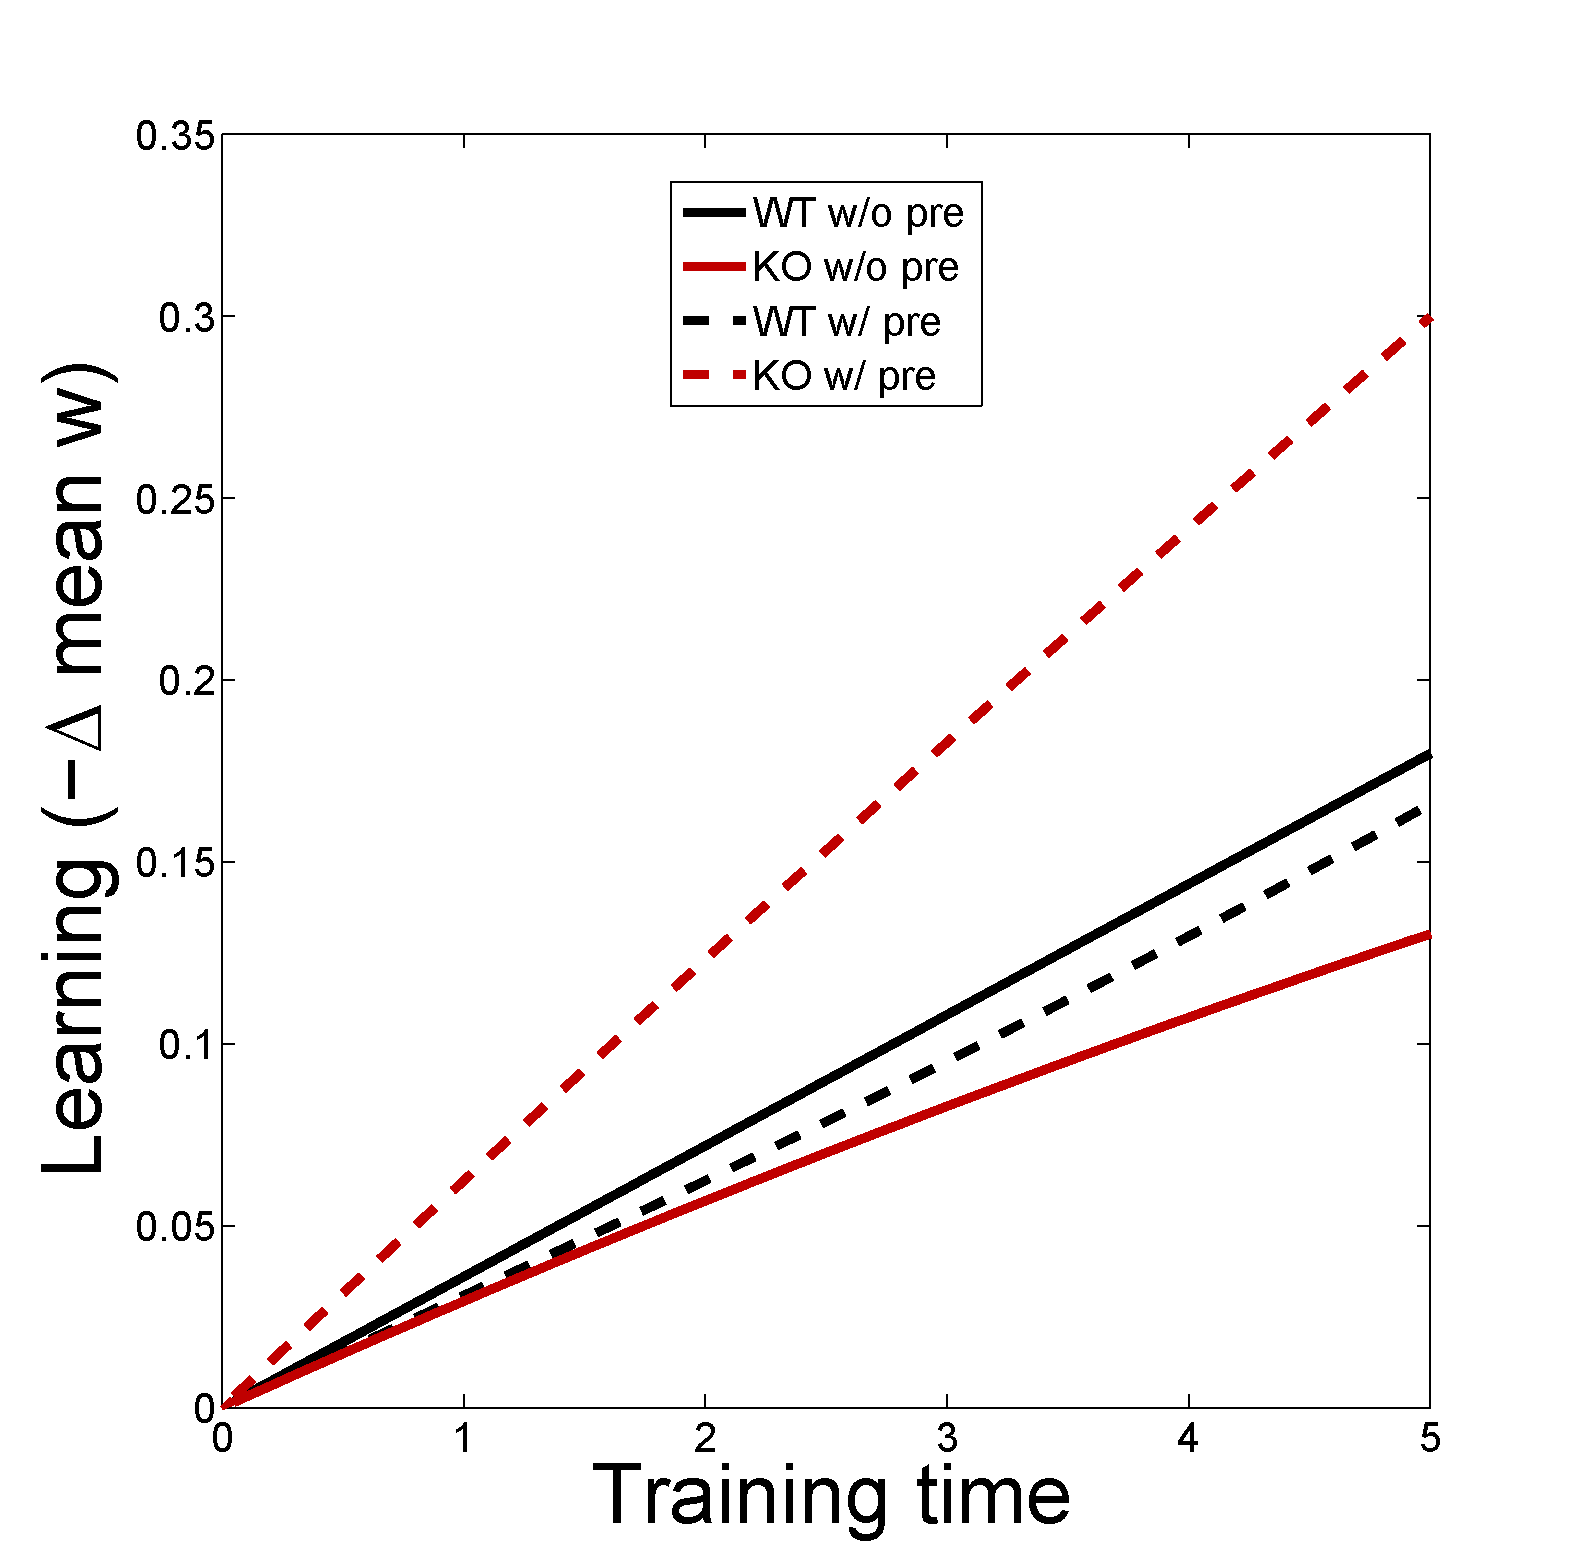
\includegraphics[width=0.35\linewidth]{serial_learnS.eps}}
   \hspace{2cm}
   \aligntop{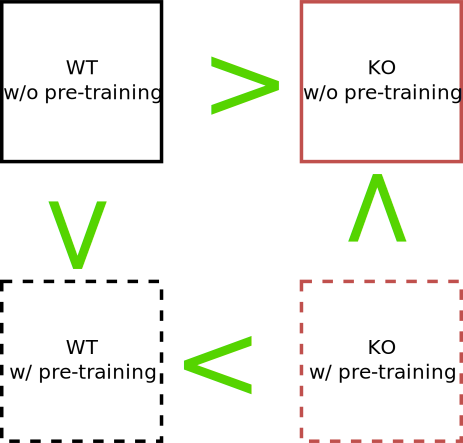
\includegraphics[width=0.35\linewidth]{comparisons_serial.svg}}
 \end{center}
 %
 \note[item]{understand why next slide}
%
\end{frame}

%-------------Slide--------------------------------------------------------

\begin{frame}{Serial synapse: initial distributions}
%
 %
 \begin{center}
 \begin{tabular}{ll}
   \aligntop{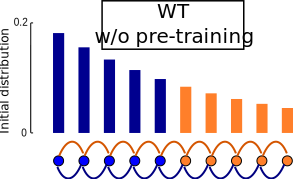
\includegraphics[height=0.2\linewidth]{serial_bar_wt_wo.svg}}
   \hspace{1cm} &
   \aligntop{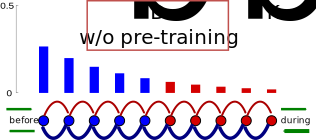
\includegraphics[height=0.2\linewidth]{serial_bar_ko_wo.svg}}
   \\[3cm]
   \aligntop{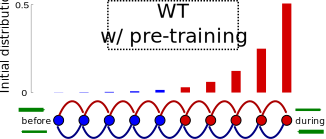
\includegraphics[height=0.2\linewidth]{serial_bar_wt_w.svg}}
   &
   \aligntop{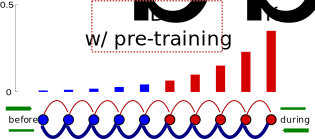
\includegraphics[height=0.2\linewidth]{serial_bar_ko_w.svg}}
 \end{tabular}
 \end{center}
 %
 \note[item]{understand why next slide}
%
\end{frame}


%-------------Slide--------------------------------------------------------

\begin{frame}{Mathematics}
%
 Serial synapse: $\eq_i \sim \CN \prn{\frac{q\pot}{q\dep}}^i$.
 
 \vp Learning rate $\sim \eq_{M/2}\prn{\frac{q\dep}{q\pot}} = \CN \prn{\frac{q\pot}{q\dep}}^{\frac{M}{2}-1}$.
 
 \vp For $M>2$, larger $q\dep \implies$ slower learning.
 
 \vp For $M=2$, larger $q\dep \implies$ larger $\CN \implies$ faster learning.
%
\end{frame}

%-------------Slide--------------------------------------------------------

\begin{frame}{Essential features}
%
 The success od the serial model relies on two features:
 \begin{itemize}
   \item Enhancing the effect of saturation,
   \note[item]{due to exponential decay}
   \item Metaplasticity -- repeated potentiation makes subsequent depression harder.
   \note[item]{push away from boundary where signal generated}
 \end{itemize}
 %
 \begin{center}
   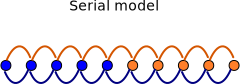
\includegraphics[width=0.4\linewidth]{serial.svg}
 \end{center}
 %
 \note[item]{borne out by other models that fail/succeed}
%
\end{frame}

%-------------Slide--------------------------------------------------------

\begin{frame}{Other models that fail}
%
 \begin{tabular}{ll}
   % & for next tab, \\ for new line...
    \aligntop{\includegraphics[width=0.4\linewidth]{multistate.svg}}\hspace{1.5cm} &
    \aligntop{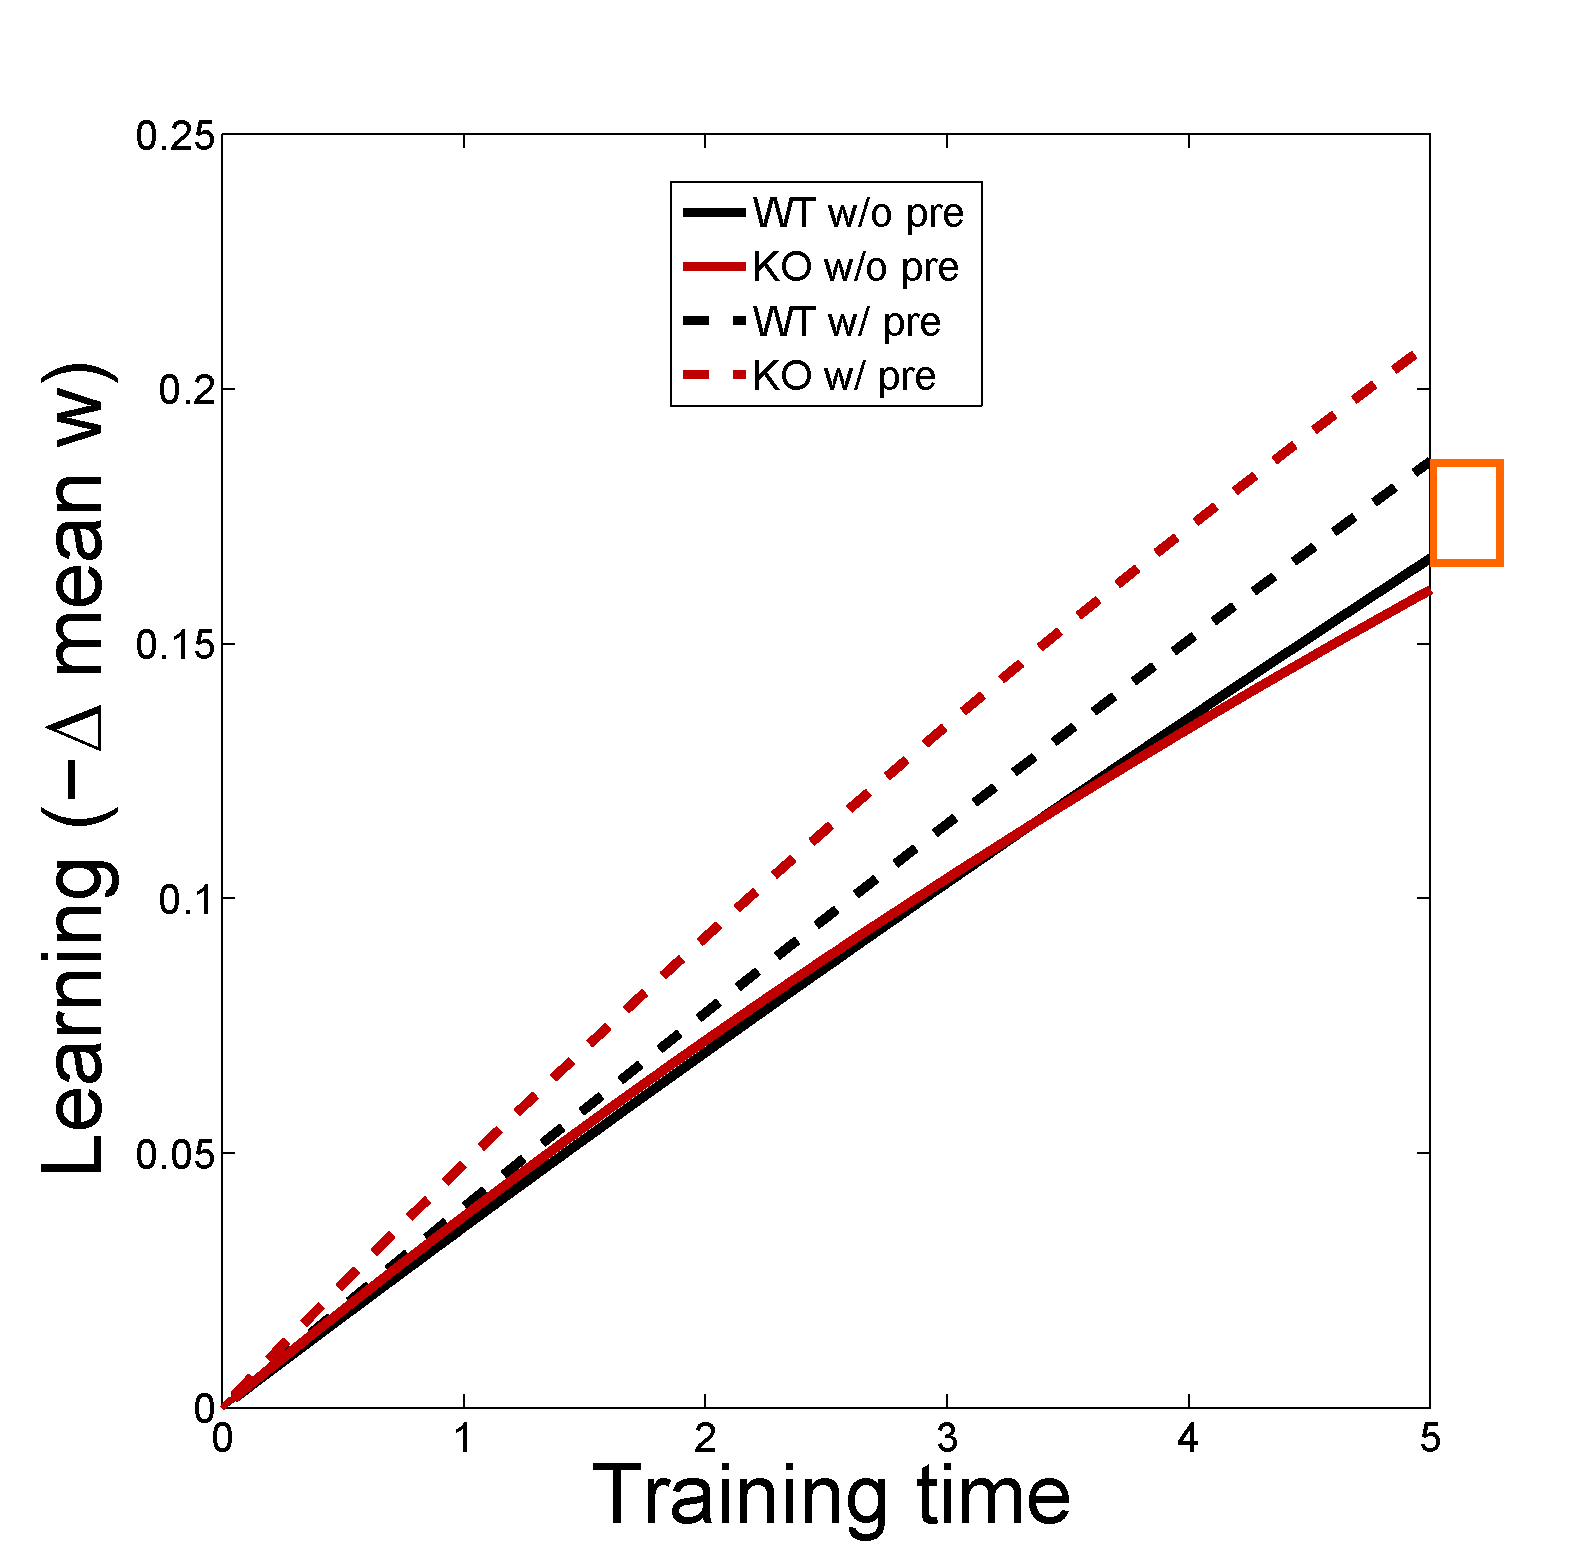
\includegraphics[width=0.28\linewidth]{multistate_learnS.eps}} \\[2cm]
    \aligntop{\includegraphics[width=0.4\linewidth]{pooled.svg}} &
    \aligntop{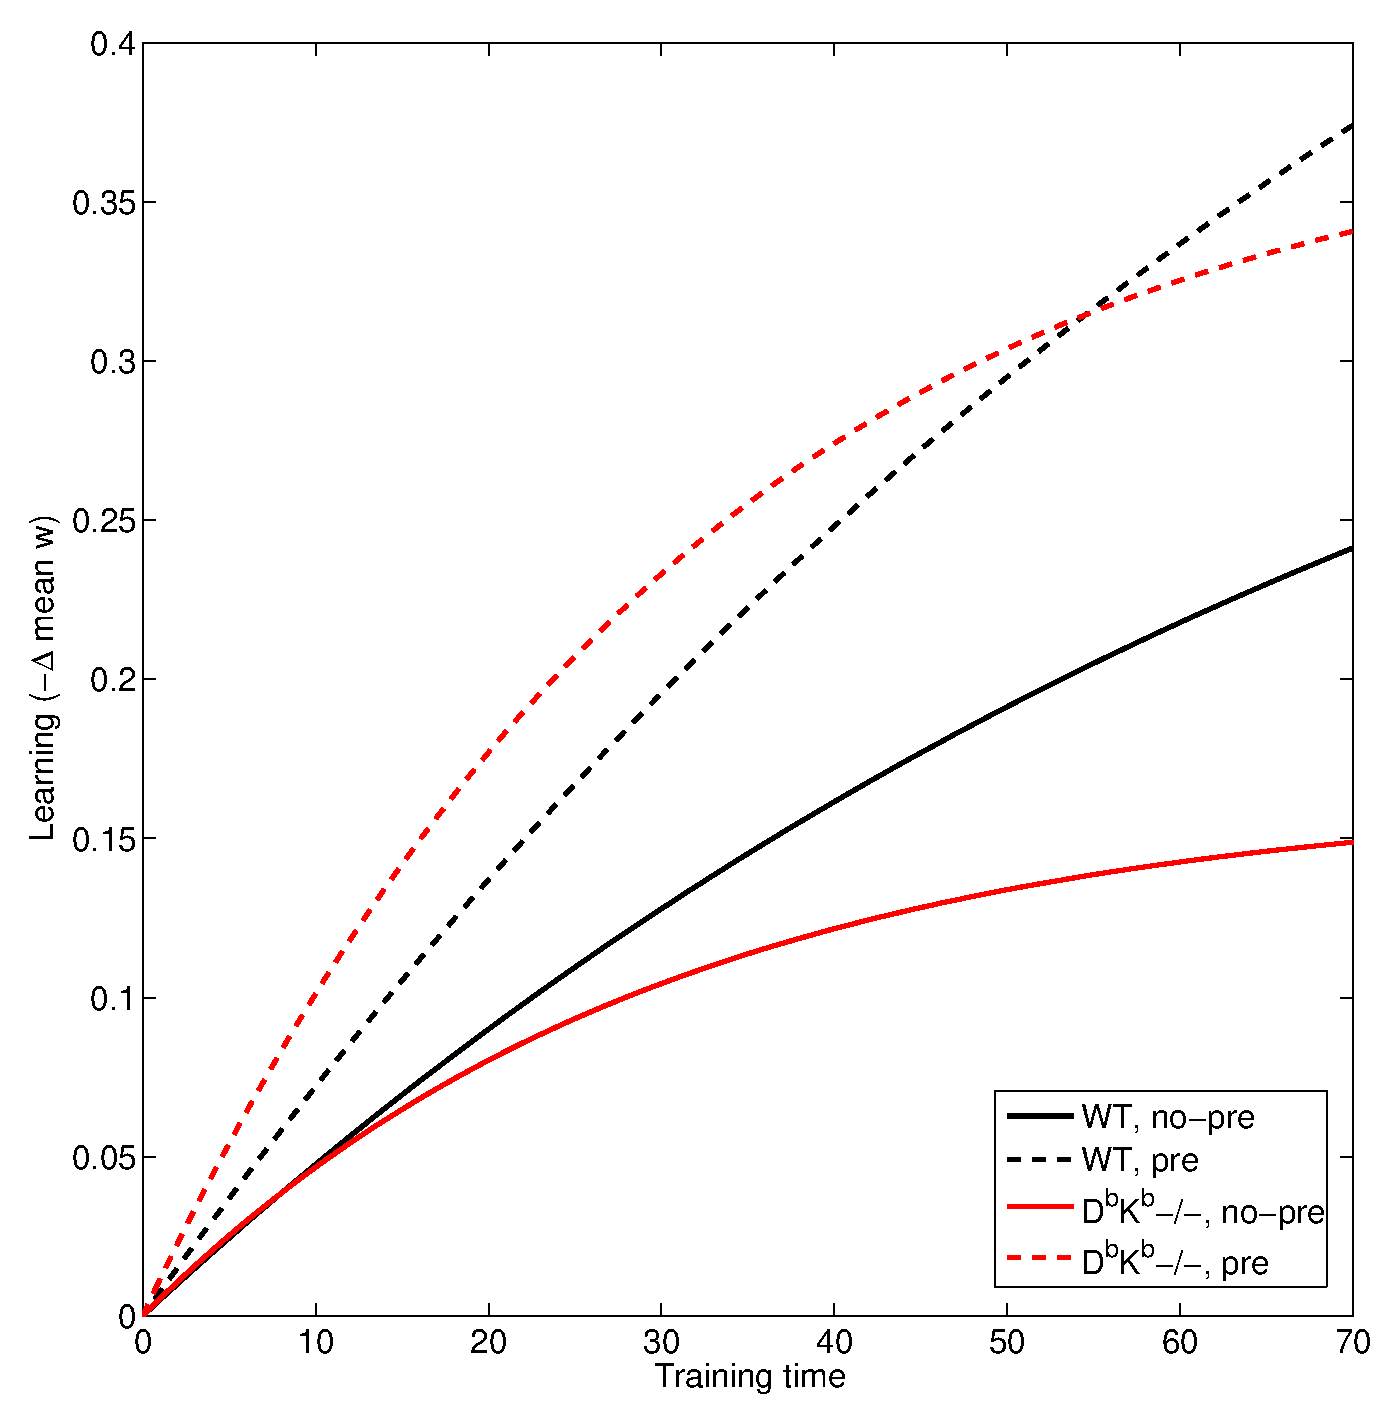
\includegraphics[width=0.28\linewidth]{pooled_scarce_learnS.eps}}
 \end{tabular}
 
 \citerr{amit1994learning}
%
\end{frame}

%-------------Slide--------------------------------------------------------

\begin{frame}{Other models that work}
%
 \begin{tabular}{ll}
   % & for next tab, \\ for new line...
    \aligntop{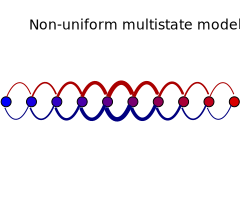
\includegraphics[width=0.4\linewidth]{multistate_nonuni.svg}}\hspace{1.5cm} &
    \aligntop{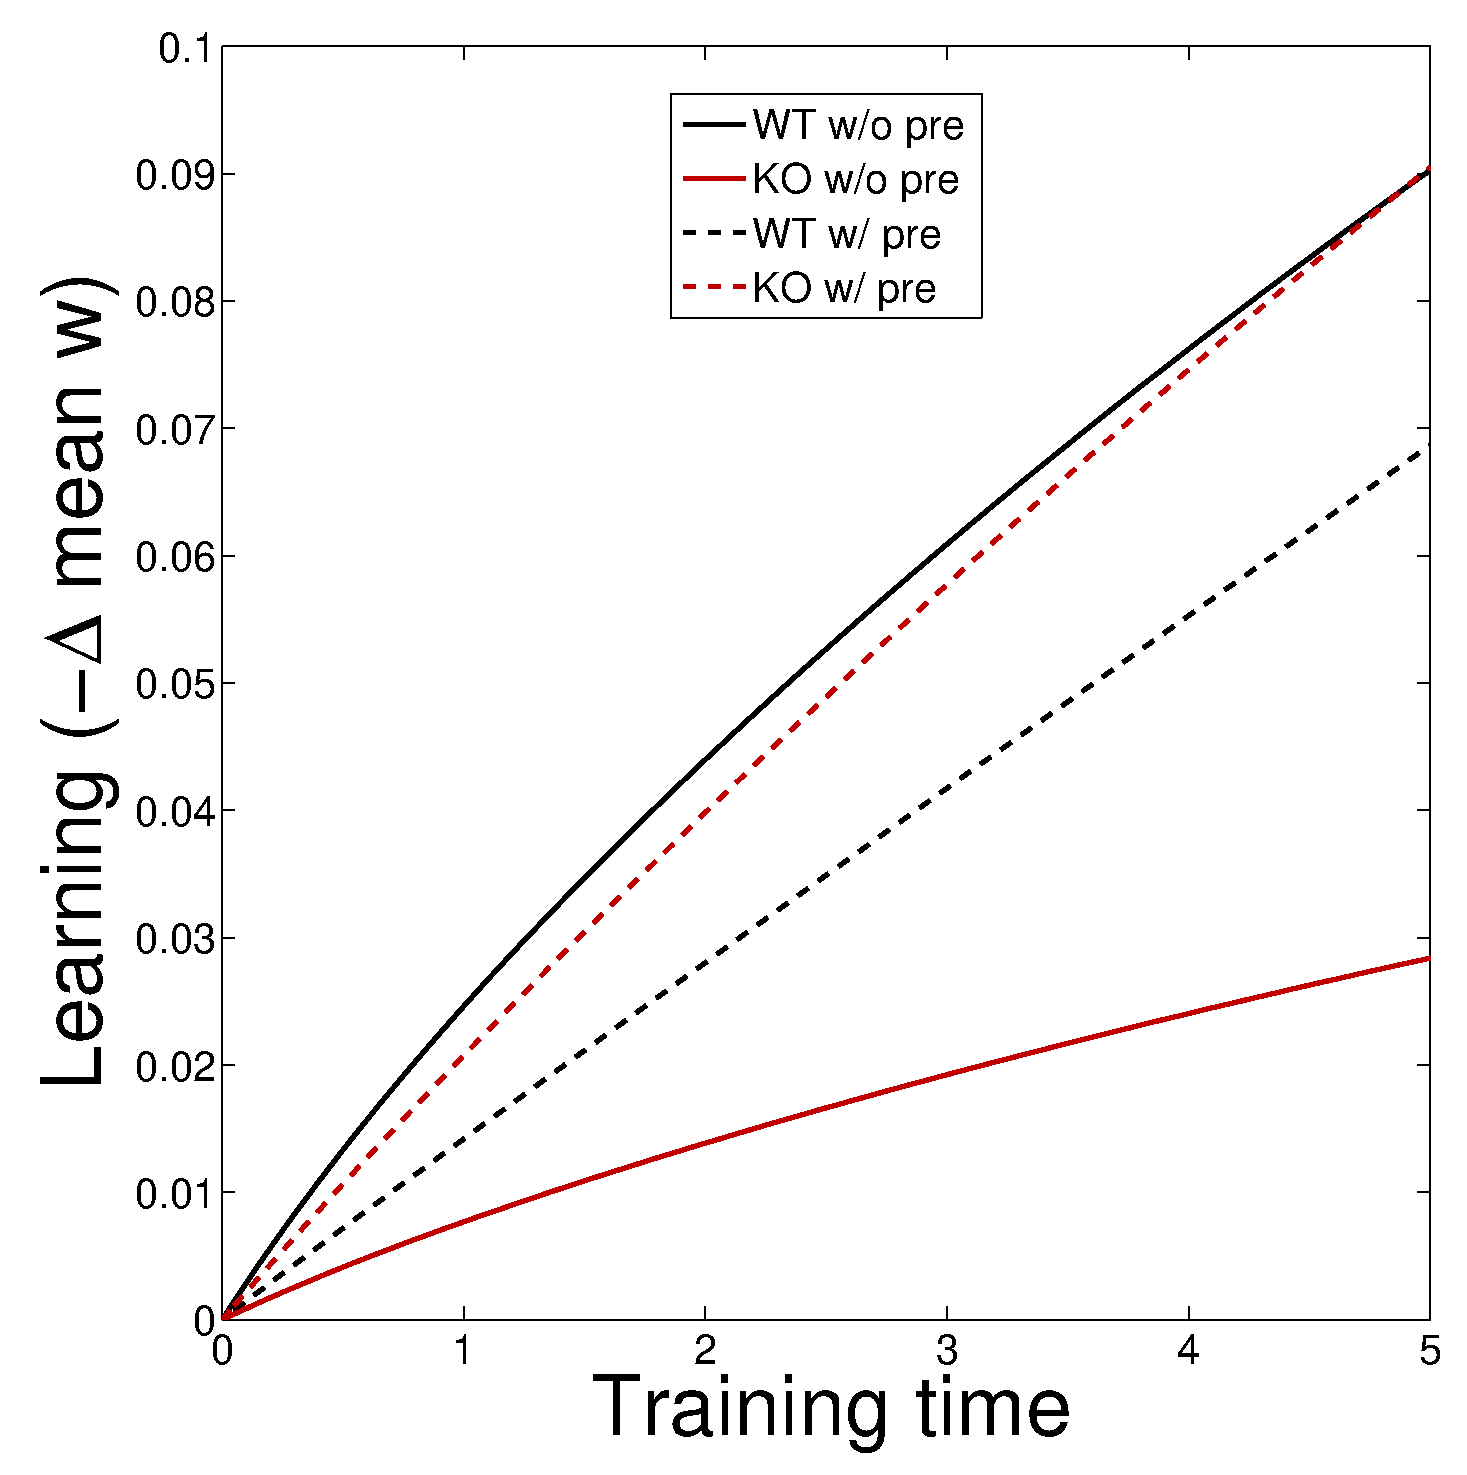
\includegraphics[width=0.28\linewidth]{nonuni_learnS.eps}} \\[2cm]
    \aligntop{\includegraphics[width=0.4\linewidth]{cascade.svg}} &
    \aligntop{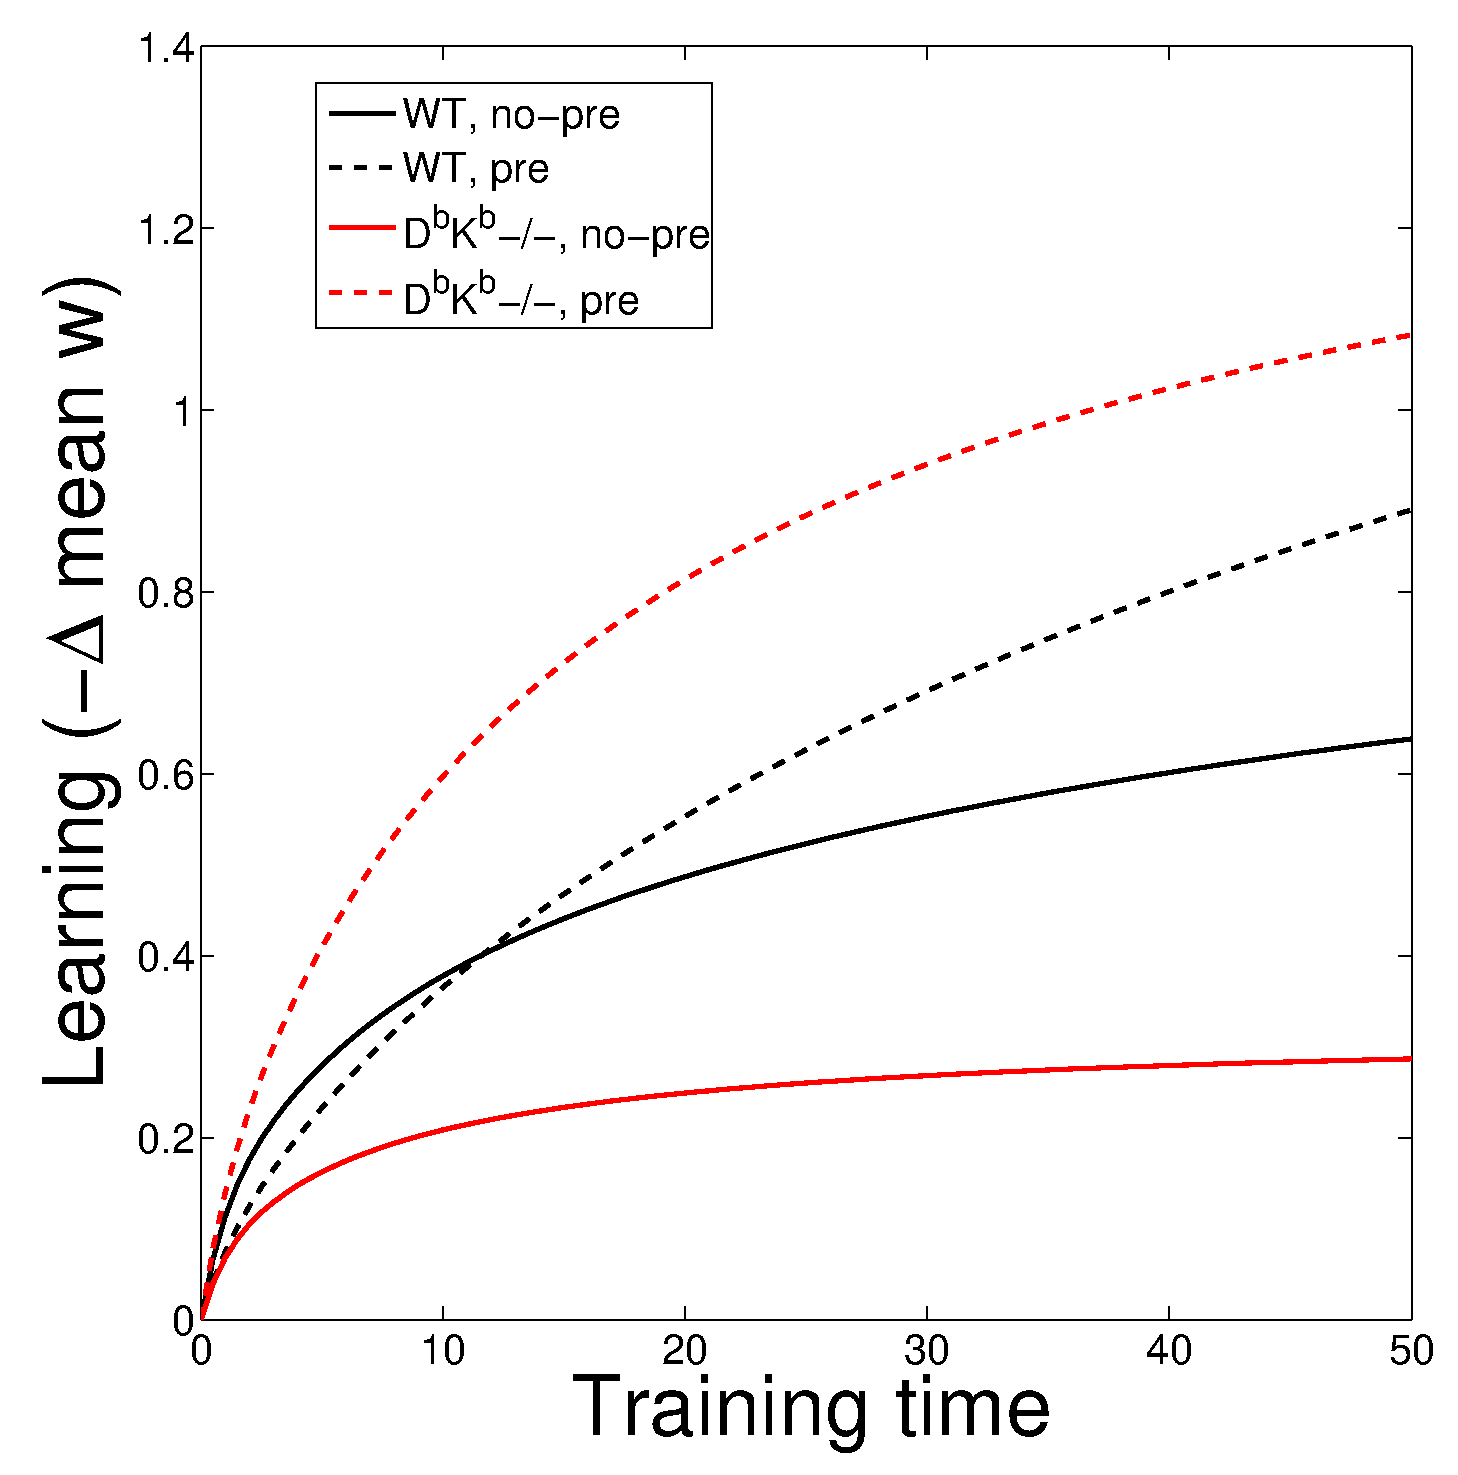
\includegraphics[width=0.28\linewidth]{cascade_long_learnS.eps}}
 \end{tabular}
 
 \citerr{Fusi2005cascade}
%
\end{frame}

%-------------Slide--------------------------------------------------------

\begin{frame}[allowframebreaks]{References}
%

 {\small
 \bibliographystyle{unsrt_slides}
 \bibliography{maths,neuro}
 }
%
\end{frame}


%-----End----------------------------------------------------------------

\end{document}

